%%%%%%%%%% Merge with supplemental materials %%%%%%%%%%
\pagebreak
% \widetext
\begin{center}
\textbf{\large Supplementary Material for Hemodynamic Deconvolution Demystified: Sparsity-Driven Regularization at Work}
\end{center}
%%%%%%%%%% Merge with supplemental materials %%%%%%%%%%
%%%%%%%%%% Prefix a "S" to all equations, figures, tables and reset the counter %%%%%%%%%%
\setcounter{equation}{0}
\setcounter{figure}{0}
\setcounter{table}{0}
\setcounter{page}{1}
\makeatletter
\renewcommand{\theequation}{S\arabic{equation}}
\renewcommand{\thefigure}{S\arabic{figure}}
\renewcommand{\bibnumfmt}[1]{[S#1]}
\renewcommand{\citenumfont}[1]{S#1}
%%%%%%%%%% Prefix a "S" to all equations, figures, tables and reset the counter %%%%%%%%%%


\begin{figure*}[h!]
    \begin{center}
        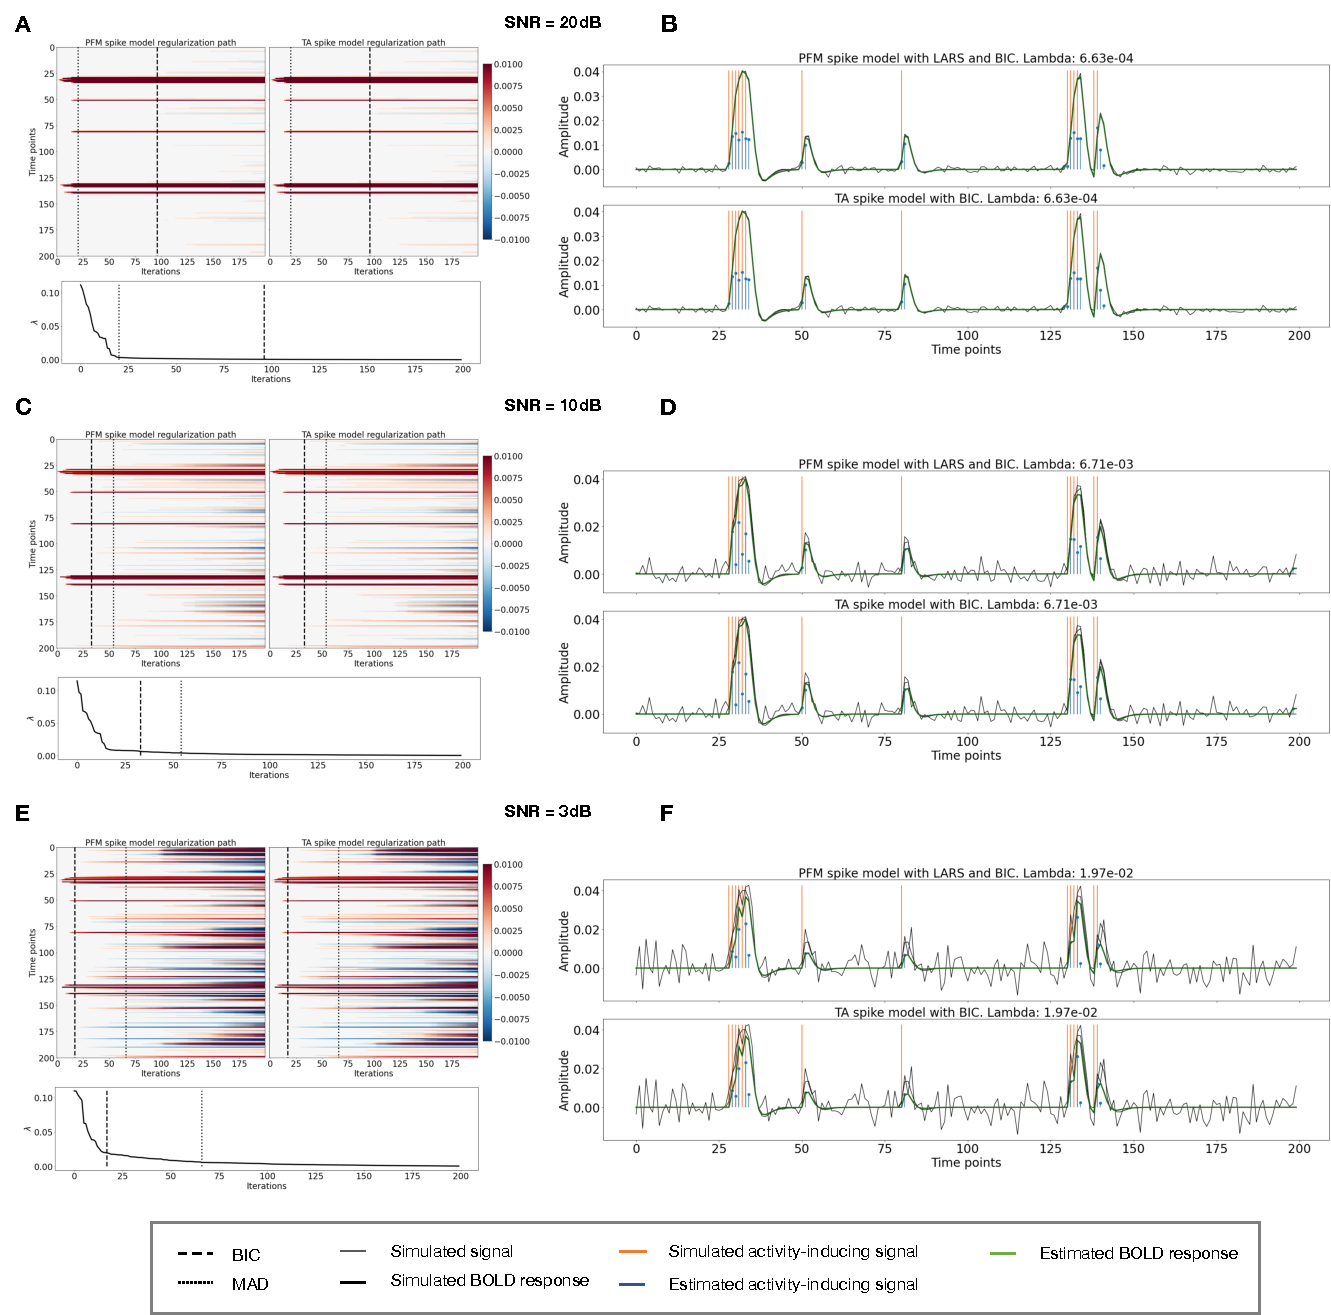
\includegraphics[width=\textwidth]{figures/regpath_spike.pdf}
    \end{center}
    \caption{Spike model simulations. (Left) Heatmap of the regularization paths of the activity-inducing signal estimated with PFM and TA as a function of \(\lambda\) (increasing number of iterations in x-axis), whereas each row in the y-axis shows one time-point. Vertical lines denote iterations corresponding to the Akaike and Bayesian Information Criteria (AIC and BIC) optima. (Right) Estimated activity-inducing (blue) and activity-related (green) signals when set based on BIC. All estimates of are identical, regardless of SNR.}
\label{fig:path_spike}
\end{figure*}

\begin{figure*}[h!]
    \begin{center}
        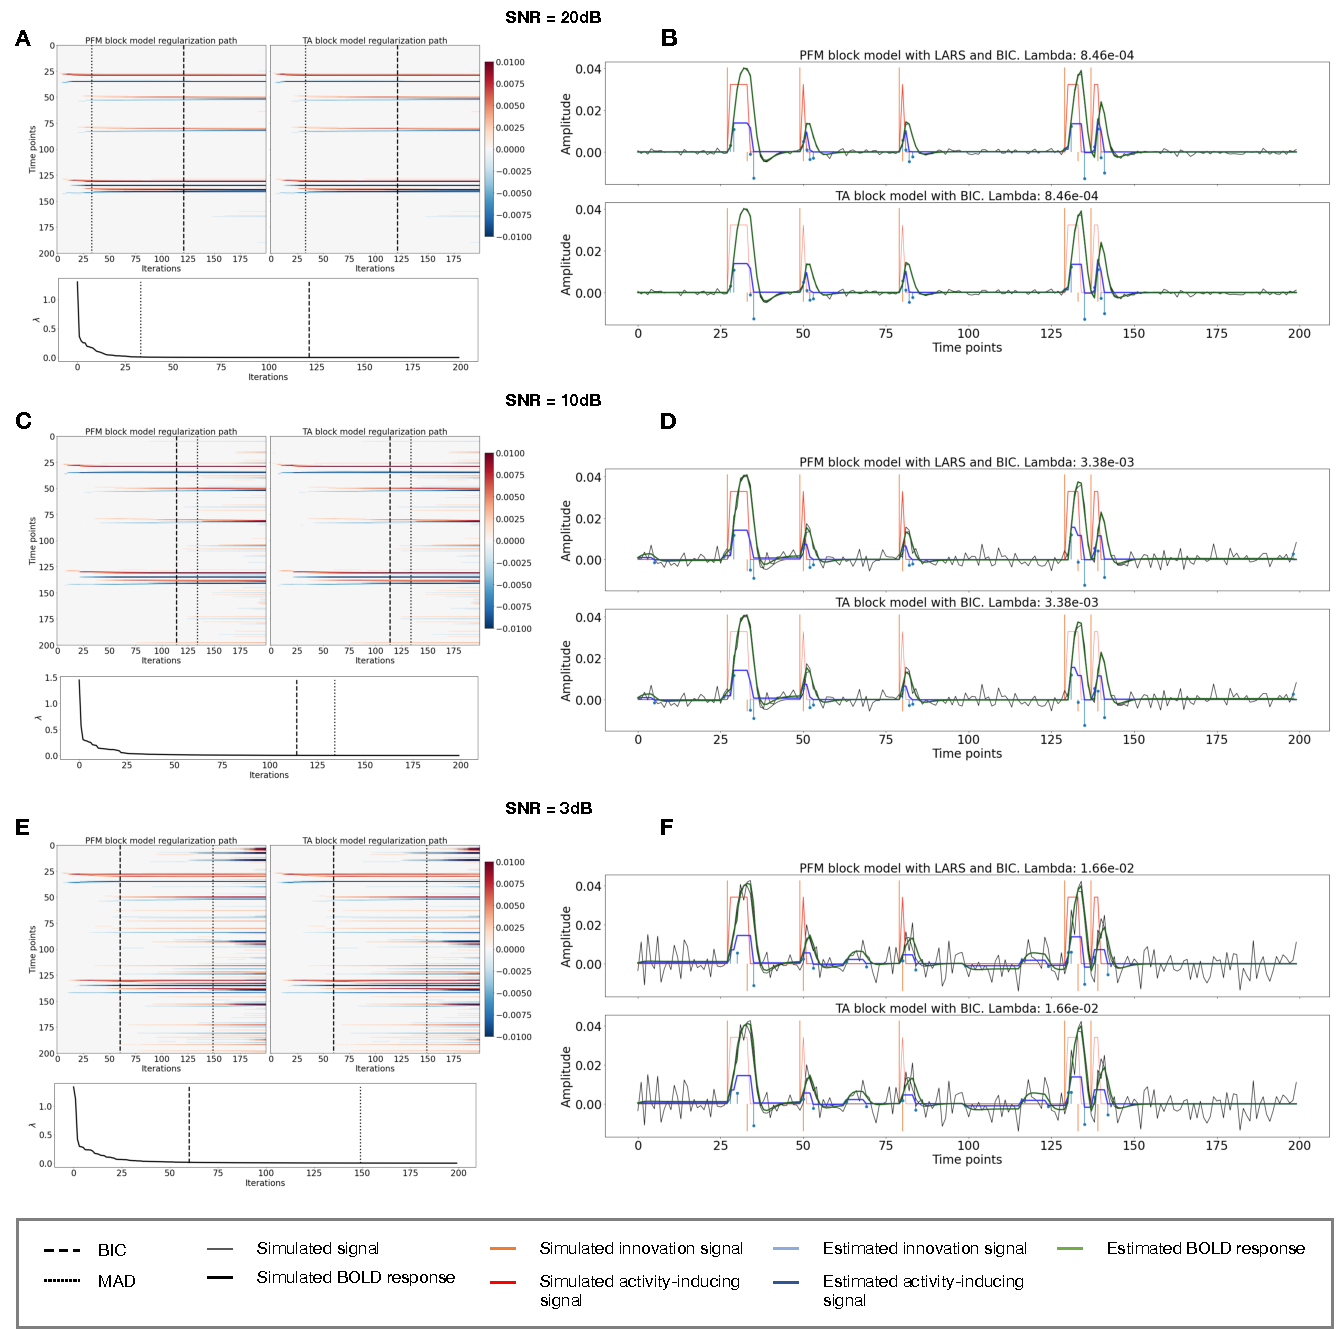
\includegraphics[width=\textwidth]{figures/regpath_block.pdf}
    \end{center}
    \caption{Block model simulations. (Left) Heatmap of the regularization paths of the innovation signal estimated with PFM and TA as a function of \(\lambda\) (increasing number of iterations in x-axis), whereas each row in the y-axis illustrates one time-point. Vertical lines denote iterations corresponding to the Akaike and Bayesian Information Criteria (AIC and BIC) optima. (Right) Estimated innovation (blue) and activity-related (green) signals when is set based on BIC. All the estimates are identical when compared between the PFM and TA cases, regardless of SNR.}
\label{fig:path_block}
\end{figure*}

% \begin{figure*}[h!]
%     \begin{center}
%         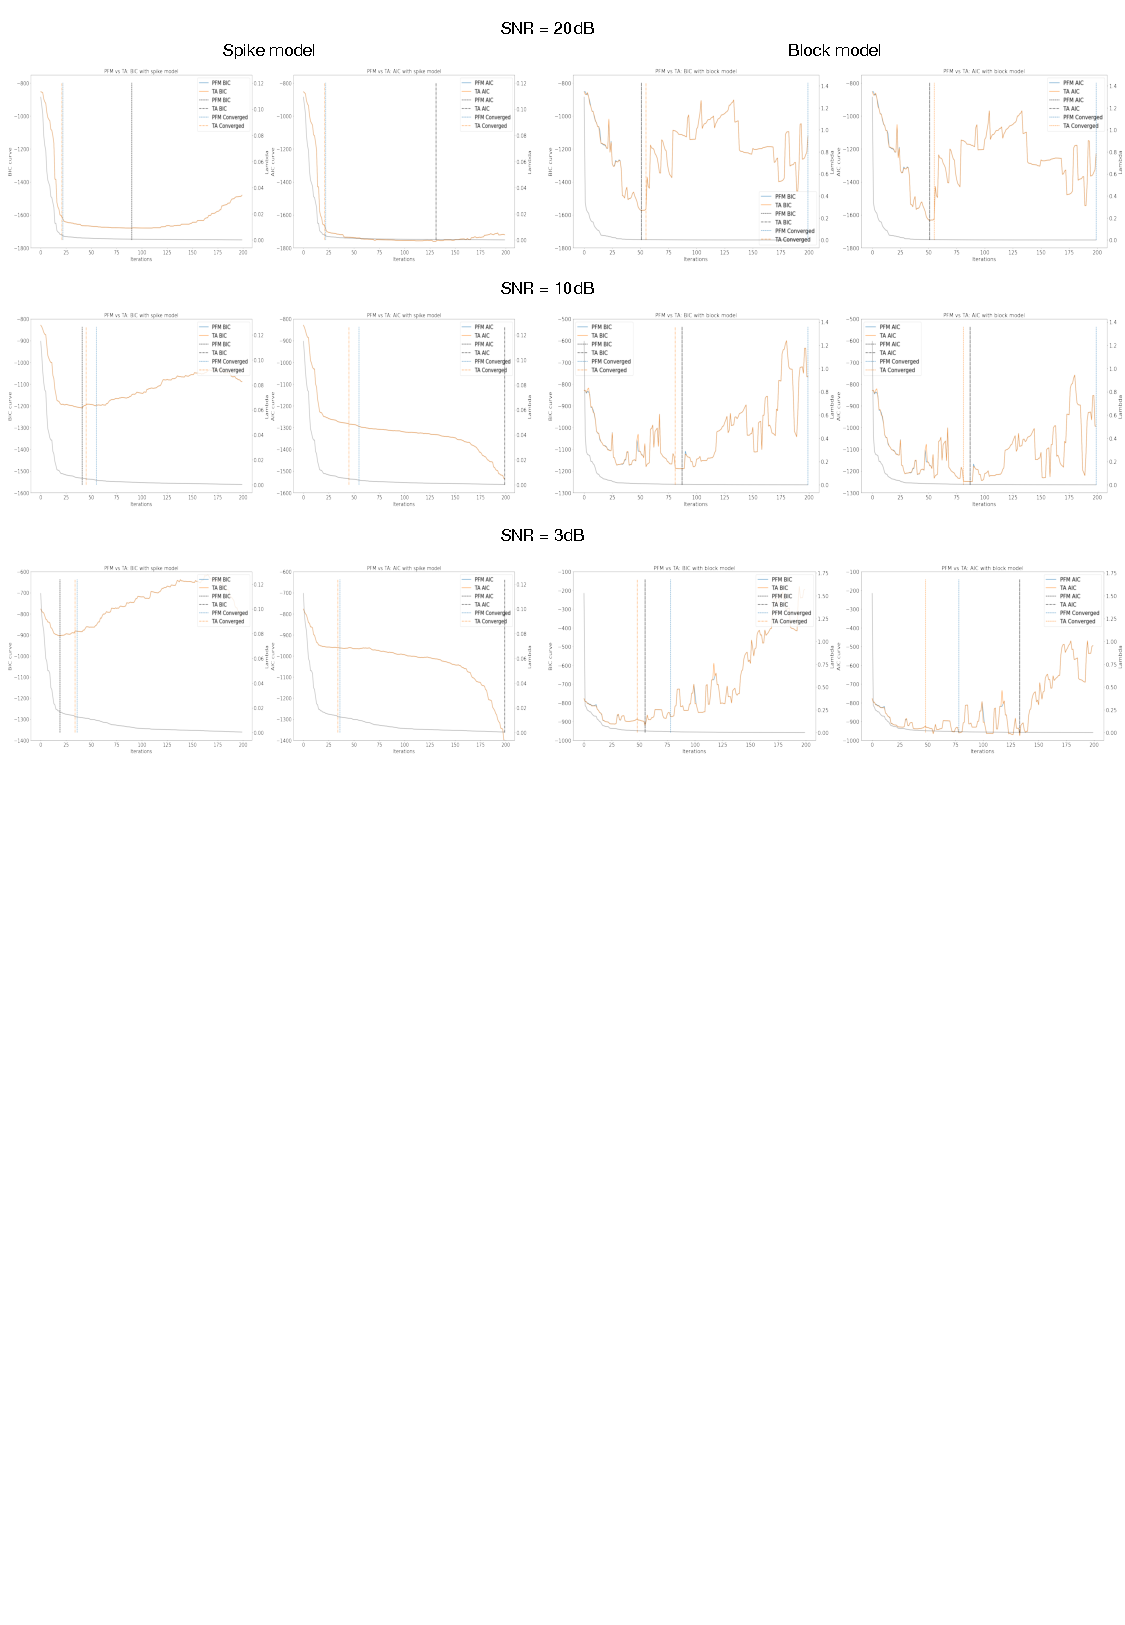
\includegraphics[width=\textwidth]{figures/lambda_cost.pdf}
%     \end{center}
%     \caption{Lambdas and cost.}
% \label{fig:lambdas}
% \end{figure*}

\begin{figure*}[h!]
    \begin{center}
        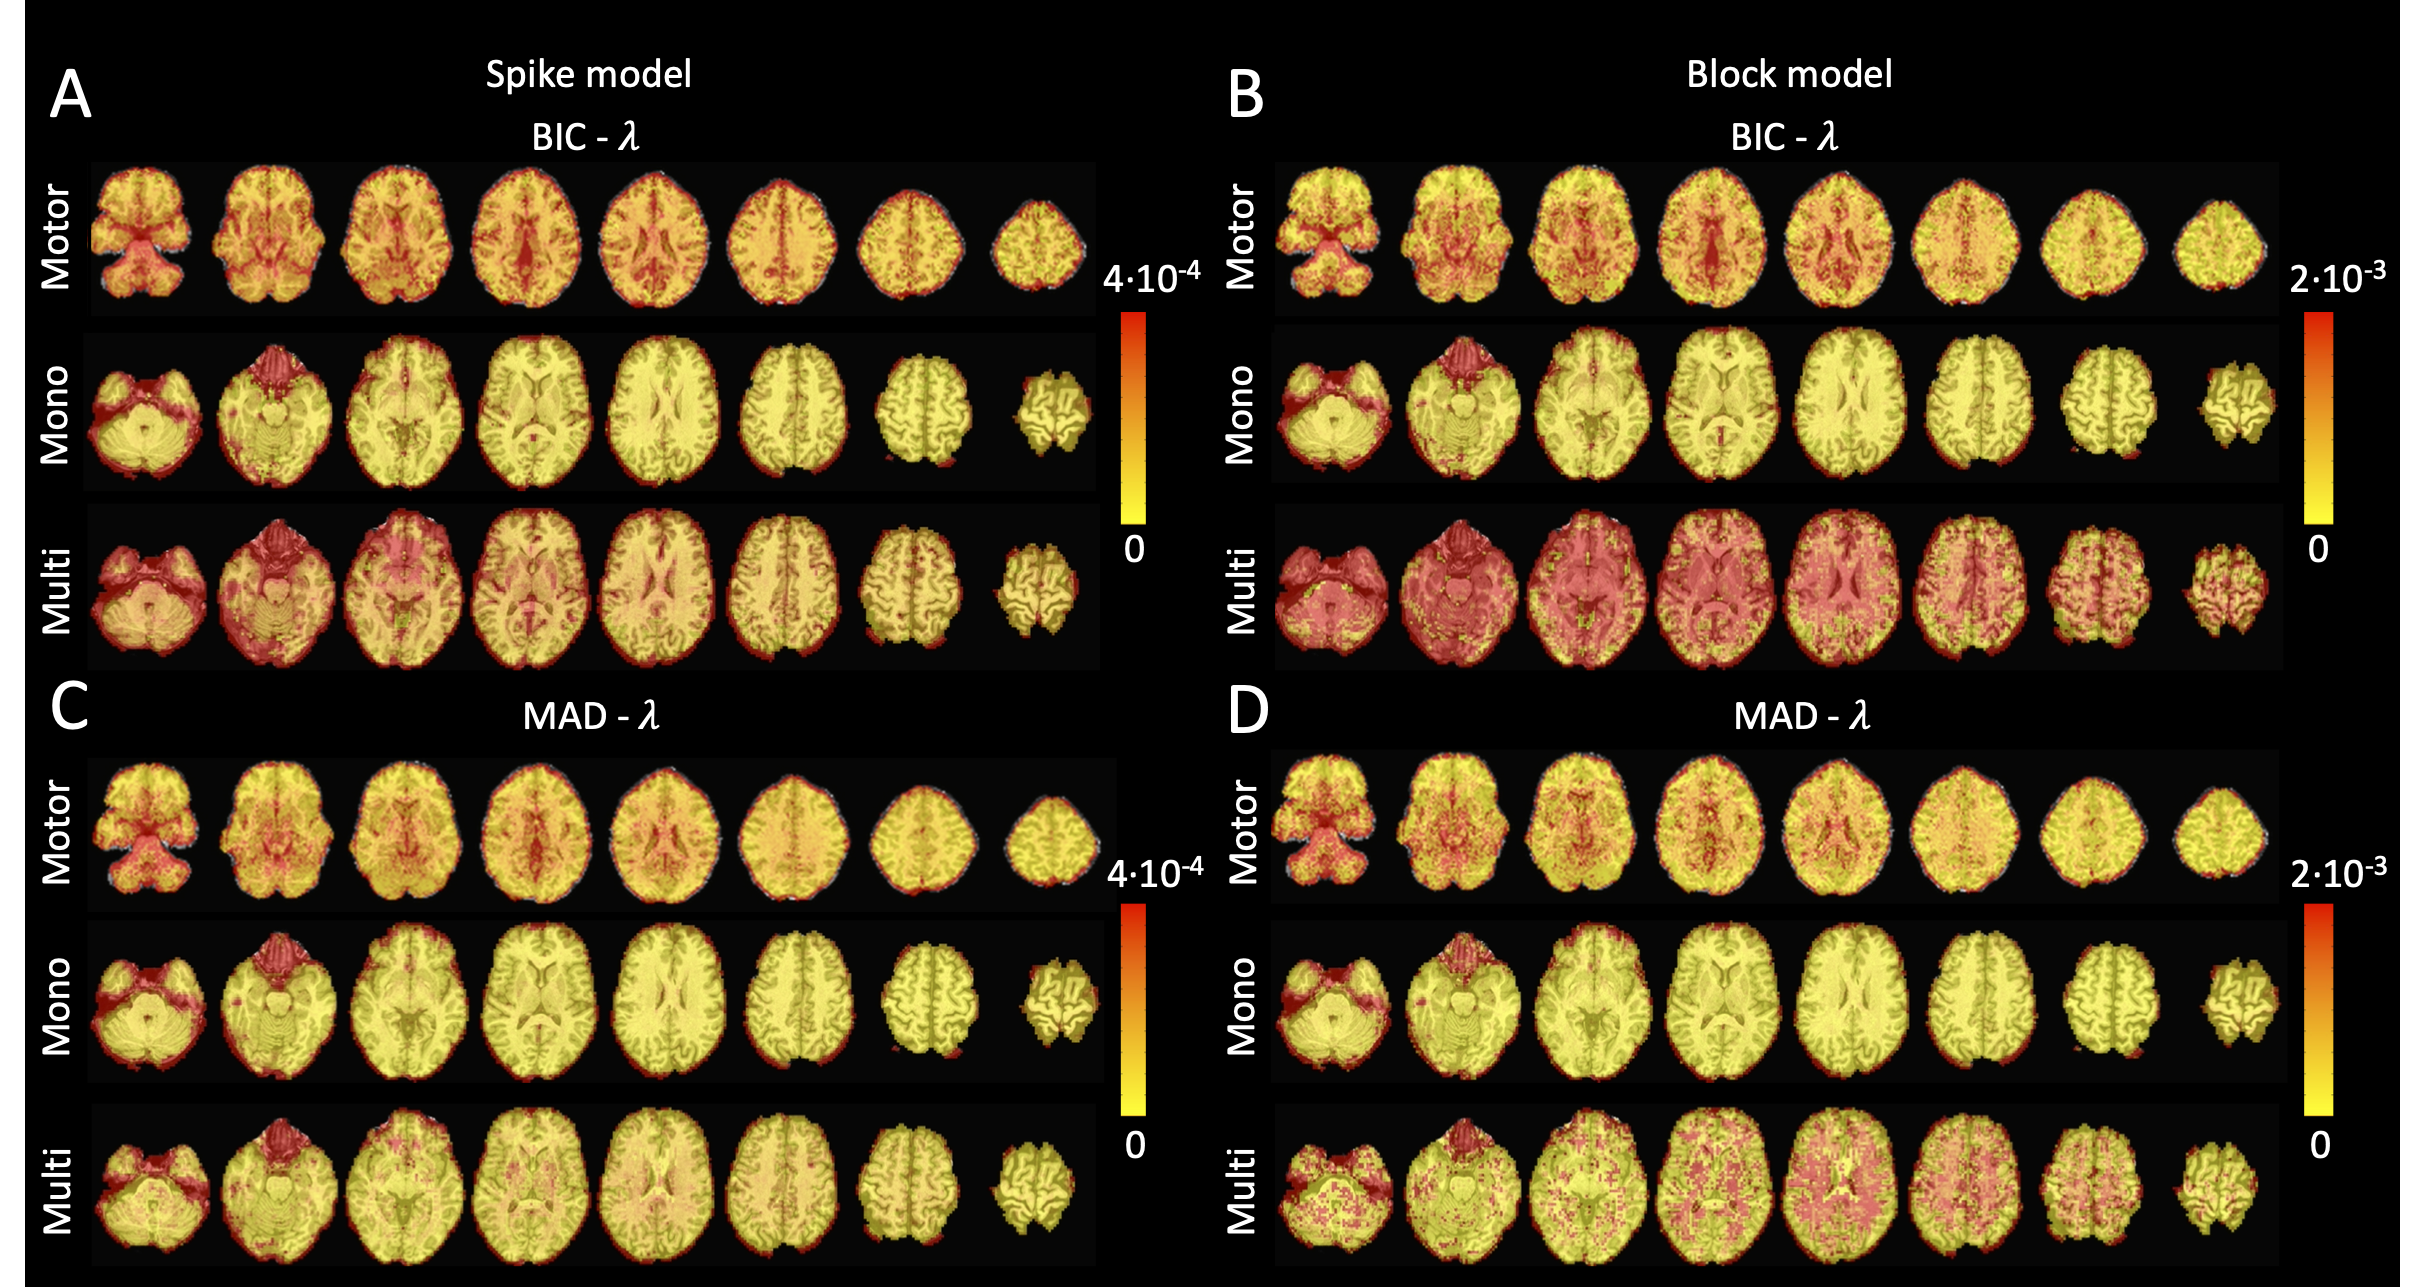
\includegraphics[width=\textwidth]{figures/supp_lambdas_map.pdf}
    \end{center}
    \caption{Lambdas.}
\label{fig:lambdas}
\end{figure*}

\begin{figure*}[h!]
    \begin{center}
        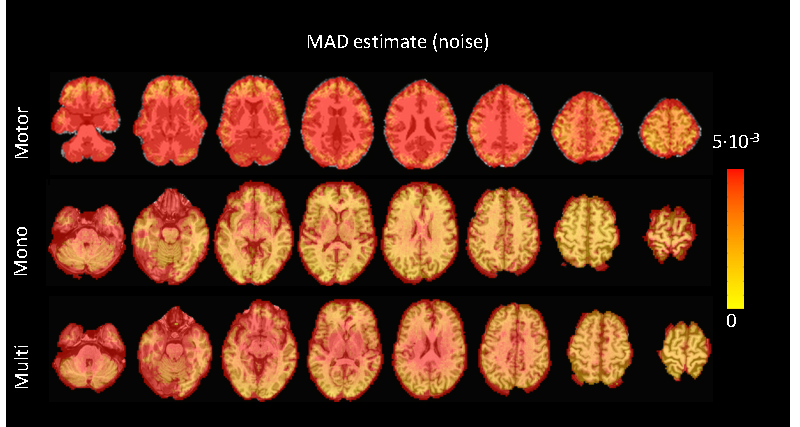
\includegraphics[width=\textwidth]{figures/supp_mad_estimate.pdf}
    \end{center}
    \caption{MAD estimate.}
\label{fig:mad_estimate}
\end{figure*}

\begin{figure*}[h!]
    \begin{center}
        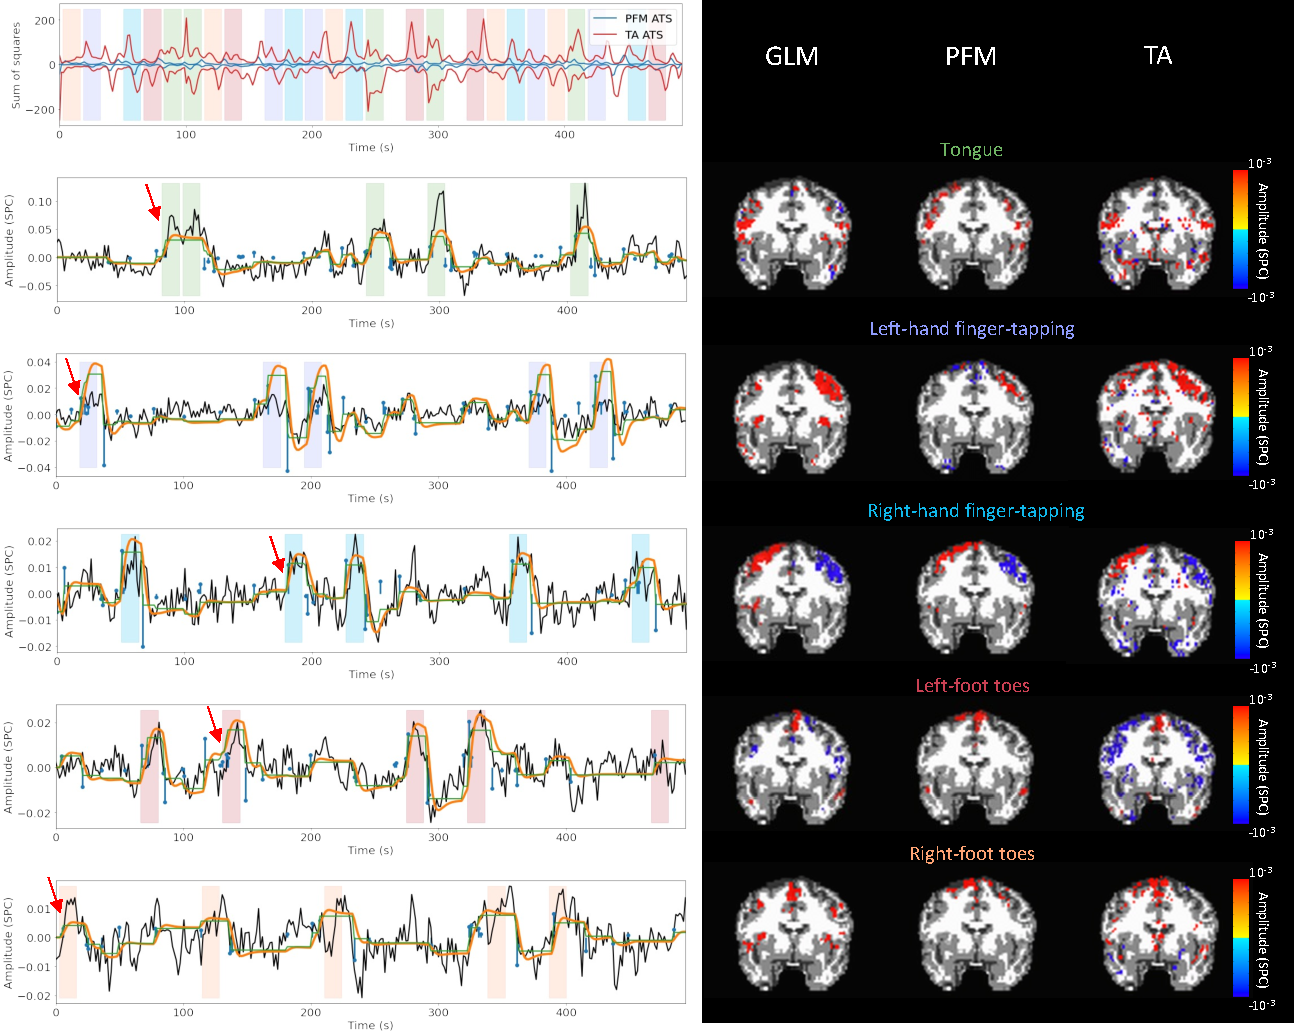
\includegraphics[width=\textwidth]{figures/supp_task_maps_mad.pdf}
    \end{center}
    \caption{Task MAD.}
\label{fig:task_mad}
\end{figure*}

\begin{figure*}[h!]
    \begin{center}
        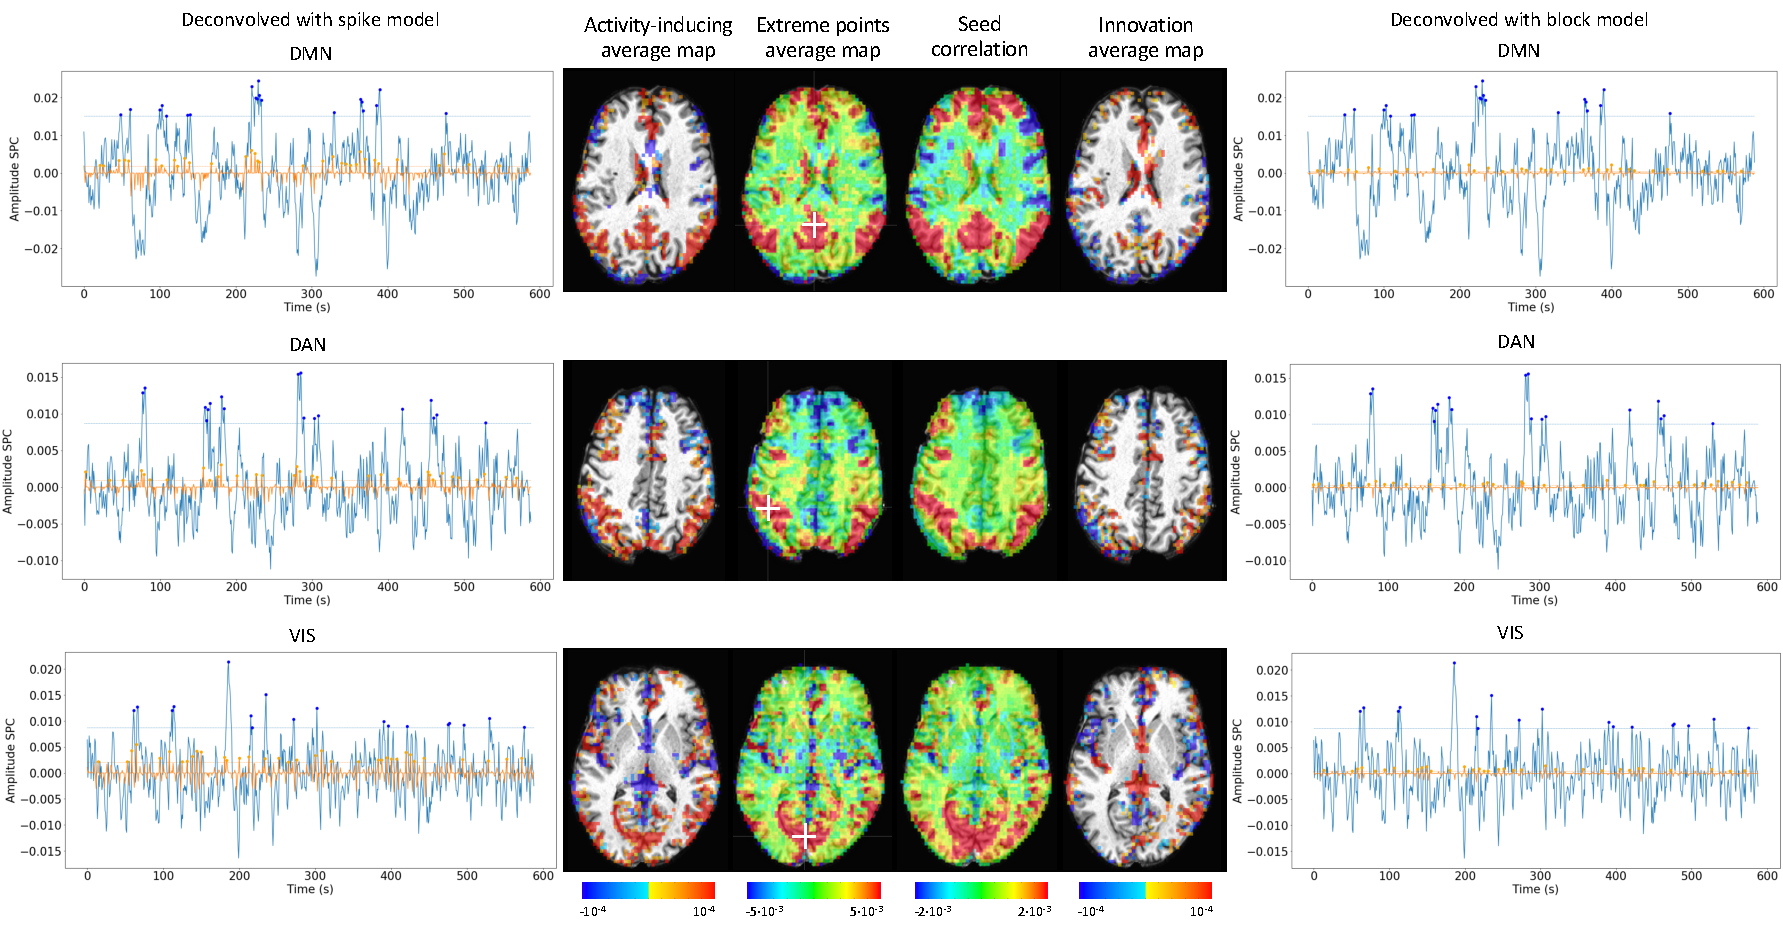
\includegraphics[width=\textwidth]{figures/supp_caps_mad.pdf}
    \end{center}
    \caption{CAPs MAD.}
\label{fig:caps_mad}
\end{figure*}